%------------------------------------------------
\begin{frame}
\frametitle{Finding the central axis}
\hypertarget{central_axis}{}
\begin{columns}[c] % The "c" option specifies centered vertical alignment while the "t" option is used for top vertical alignment

\column{.3\textwidth} % Left column and width

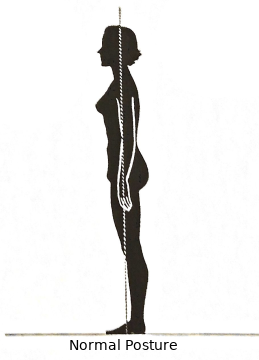
\includegraphics[width=\linewidth]{Normal_Posture}

\column{.7\textwidth} % Left column and width
\structure{Stand up} straight and close your eyes. Imagine a \structure{stream of energy} flowing between your feet upwards, through your body (central axis). Feel how your skeleton, how your musculature and their tissues and the organs \structure{organize themselves around this central axis}. Everything is in movement. Take your time, allow changes to happen even to the cellular level.

Start \structure{turning} around the axis with little steps, one way, then the other. \structure{Repeat}. Then stop and \structure{orient yourself} in this position, correct yourself if necessary. Feel again the sensation of this central axis.
\end{columns}

\end{frame}
%------------------------------------------------
%------------------------------------------------
\begin{frame}
\frametitle{Finding the central axis - when and why}
\hypertarget{central_axis}{}
\begin{columns}[c] % The "c" option specifies centered vertical alignment while the "t" option is used for top vertical alignment

\column{.3\textwidth} % Left column and width

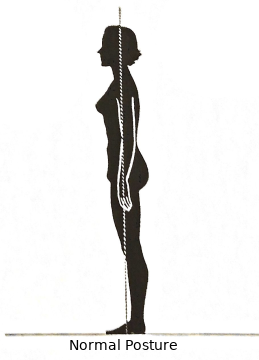
\includegraphics[width=\linewidth]{Normal_Posture}

\column{.7\textwidth} % Left column and width
You may add this exercise to your \structure{morning program}. Or practice it when you feel that you fell out of your \structure{center}. Enjoy this feeling of the central axis and take it into your day.

\structure{Actively registering} what you feel accelerates your progress. It happens completely from your \structure{feelings} and there's no need for perfection. Your new \structure{perception of your body} will stay this way more present and you will be able to \structure{build on it} as a foundation. Give your body the time needed, be \structure{affectionate} with it and celebrate every progress.
\end{columns}

\end{frame}
%------------------------------------------------
